% =====================================================================
%  Relatório do projeto — formato SBC (Sociedade Brasileira de Computação)
%
%  Este arquivo é AUTOCONTIDO: reproduz o estilo do template oficial da SBC
%  (margens, fontes Times/Helvetica/Courier, título 16pt, abstract+resumo
%  recuados 0,8cm, seções 13pt, legendas Helvetica 10pt, referências autor-data)
%  usando apenas pacotes padrão. Compila em qualquer distribuição TeX e no
%  Overleaf, SEM precisar do sbc-template.sty.
%
%  Se preferir o pacote OFICIAL da SBC (ex.: submissão a um evento), troque o
%  preâmbulo por:
%     \documentclass[12pt]{article}
%     \usepackage{sbc-template}
%     \usepackage{graphicx,url}
%     \usepackage[brazil]{babel}
%     \usepackage[utf8]{inputenc}
%  e use \title, \author, \address, \begin{document}\maketitle, \begin{abstract},
%  \begin{resumo}. O corpo (seções/tabelas/figuras/referências) abaixo é
%  reaproveitável.
%
%  As figuras referenciadas estão em ./figuras/ (este .tex fica na raiz do
%  projeto). Compile com pdflatex (2x, para resolver as referências cruzadas).
%
%  >>> EDITE os campos marcados com %% EDITE (autor, instituição, e-mail). <<<
% =====================================================================
\documentclass[12pt,a4paper]{article}

\usepackage[T1]{fontenc}
\usepackage[utf8]{inputenc}
\usepackage[brazil]{babel}
\usepackage[a4paper,top=3.5cm,bottom=2.5cm,left=3cm,right=3cm]{geometry}

\usepackage{mathptmx}              % Times (texto + matemática)
\usepackage[scaled=0.92]{helvet}  % Helvetica (legendas)
\usepackage{courier}              % Courier (e-mails)

\usepackage{amsmath}
\usepackage{graphicx}
\usepackage{booktabs}
\usepackage{url}
\usepackage[hidelinks]{hyperref}
\usepackage{titlesec}
\usepackage{caption}
\usepackage{float}

% --- layout geral conforme o template SBC ---
\pagestyle{empty}                              % sem numeração de páginas
\setlength{\parindent}{1.27cm}                 % indentação dos parágrafos
\setlength{\parskip}{0pt}
\linespread{1.02}
\emergencystretch=3em   % evita overfull \hbox em parágrafos justificados

% --- títulos de seção (13pt) e subseção (12pt), em negrito, alinhados à esq. ---
\titleformat{\section}{\normalfont\fontsize{13}{15}\bfseries}{\thesection.}{0.5em}{}
\titleformat{\subsection}{\normalfont\fontsize{12}{14}\bfseries}{\thesubsection}{0.5em}{}
\titlespacing*{\section}{0pt}{12pt}{6pt}
\titlespacing*{\subsection}{0pt}{10pt}{4pt}

% --- legendas: Helvetica, 10pt, negrito, "Figura 1." ---
\captionsetup{font={footnotesize,bf,sf},labelsep=period,justification=centering}

% --- ambiente para abstract / resumo (recuo de 0,8cm dos dois lados) ---
\newenvironment{sbcabstract}
  {\par\vspace{6pt}\begingroup\setlength{\leftskip}{0.8cm}\setlength{\rightskip}{0.8cm}\noindent}
  {\par\endgroup\vspace{6pt}}

% --- item de referência: 1a linha à margem, demais recuadas 0,5cm, 6pt antes ---
\newcommand{\refitem}[1]{\par\vspace{6pt}\noindent\hangindent=0.5cm\hangafter=1 #1\par}

\begin{document}

% =====================================================================
%  PRIMEIRA PÁGINA: título, autores, endereço, abstract e resumo
% =====================================================================
\begin{center}
  {\fontsize{16}{19}\selectfont\bfseries
   Espacialização da evapotranspiração de referência (ET\textsubscript{0})
   diária: reprodução de Baratto et al.\ (2022) e contribuição com krigagem,
   RFRK e teste de Wilcoxon\par}

  \vspace{12pt}
  {\fontsize{12}{14}\selectfont\bfseries
   Antonio Albuquerque de Oliveira Neto\textsuperscript{1},
   Gabriel Antônio de Oliveira Rocha\textsuperscript{1}\par}

  \vspace{12pt}
  {\fontsize{12}{14}\selectfont
   \textsuperscript{1}Recife -- PE -- Brasil\par}

  \vspace{6pt}
  {\footnotesize\ttfamily \{aaon, gaor\}@cesar.school\par}
\end{center}

\vspace{12pt}

\begin{sbcabstract}
\noindent\textbf{Abstract.}\textit{ This work reproduces the comparison of daily
reference-evapotranspiration (ET\textsubscript{0}) interpolators by Baratto et
al.\ (2022) --- IDW (powers 1--5), ADW and Random Forest (RF) --- evaluated by
leave-one-out cross-validation (LOO-CV) with Willmott's $d$, RMSE, BIAS and MAE,
over 12 automatic INMET stations in Espírito Santo, Brazil (2023). We add four
elements absent from the original study: ordinary kriging (OK) as a geostatistical
benchmark, Random Forest Regression Kriging (RFRK), a paired Wilcoxon test, and an
RF variable-importance analysis. The interpolators are nearly indistinguishable
(RF leads $d$/RMSE/MAE by a negligible margin). Wilcoxon shows that the
``significant'' differences are practically irrelevant ($\approx$0.008~mm/day);
RFRK removes RF's blocky artifacts with lower bias; and variable importance reveals
that RF's skill is mostly seasonal (day-of-year $\approx$0.87), not spatial. The
pipeline is packaged with CLI, MLflow, a Streamlit dashboard and Docker.}
\end{sbcabstract}

\begin{sbcabstract}
\noindent\textbf{Resumo.}\textit{ Este trabalho reproduz a comparação de
interpoladores de evapotranspiração de referência (ET\textsubscript{0}) diária de
Baratto et al.\ (2022) --- IDW (potências 1--5), ADW e Random Forest (RF) ---
avaliada por validação cruzada \emph{leave-one-out} (LOO-CV) com o índice $d$ de
Willmott, RMSE, BIAS e MAE, sobre 12 estações automáticas do INMET no Espírito
Santo (2023). Acrescentam-se quatro elementos ausentes do estudo original: a
krigagem ordinária (OK) como \emph{benchmark} geoestatístico, o \emph{Random
Forest Regression Kriging} (RFRK), um teste de Wilcoxon pareado e a análise de
importância de variáveis do RF. Os interpoladores são quase indistinguíveis (o RF
lidera $d$/RMSE/MAE por margem desprezível). O Wilcoxon mostra que as diferenças
``significativas'' são praticamente irrelevantes ($\approx$0,008~mm/dia); o RFRK
remove os artefatos ``em blocos'' do RF com menor viés; e a importância de
variáveis revela que a habilidade do RF é majoritariamente sazonal (dia do ano
$\approx$0,87), não espacial. O pipeline é empacotado com CLI, MLflow, painel
Streamlit e Docker.}
\end{sbcabstract}

% =====================================================================
\section{Introdução}
% =====================================================================

A evapotranspiração de referência (ET\textsubscript{0}) é uma variável central no
balanço hídrico e no manejo da irrigação, mas é medida em poucos pontos: a rede de
estações meteorológicas é esparsa frente à extensão das bacias hidrográficas. Por
isso, \emph{espacializar} a ET\textsubscript{0} --- estimar seu valor onde não há
estação, a partir das estações vizinhas --- é um problema recorrente em hidrologia
e agrometeorologia. A escolha do método de interpolação é o ponto sensível: vai do
clássico \emph{Inverse Distance Weighting} (IDW) a métodos geoestatísticos e, mais
recentemente, a aprendizado de máquina.

O trabalho de [Baratto et al.\ 2022] compara, em bacias da Mata Atlântica,
interpoladores de ET\textsubscript{0} diária --- IDW com expoentes de 1 a 5, o
\emph{Angular Distance Weighting} (ADW) e o \emph{Random Forest} (RF) --- por
validação cruzada \emph{leave-one-out} (LOO), e elege o RF como ``melhor'' método.
Há, porém, uma tensão no próprio resultado: o RF é escolhido pelo \emph{detalhe
espacial dos mapas}, embora \emph{não vença nas métricas} --- no estudo original, o
IDW de expoente alto tem o maior índice $d$ de Willmott. A escolha do ``vencedor'',
ali, é qualitativa. Além disso, o paper deixa três lacunas: (i) não inclui um
\emph{benchmark} geoestatístico (krigagem); (ii) não testa se as diferenças entre
métodos são estatisticamente significativas; e (iii) afirma a vantagem do RF mas
nunca mostra \emph{de onde} ela vem (quais variáveis o RF de fato usa).

Este trabalho tem dois objetivos. O primeiro é \textbf{reproduzir} a metodologia de
[Baratto et al.\ 2022] em outra região e período --- estações automáticas do INMET
no Espírito Santo, ano de 2023 --- verificando se o padrão central se mantém. O
segundo é \textbf{contribuir} com aquilo que o paper deixou em aberto:

\begin{enumerate}
  \item \textbf{OK} --- krigagem ordinária, o \emph{benchmark} geoestatístico
        ausente no paper;
  \item \textbf{RFRK} --- \emph{Random Forest Regression Kriging} (RF nas
        covariáveis $+$ krigagem dos resíduos), método híbrido que ataca as duas
        fraquezas do RF (perder nas métricas e gerar mapas ``em blocos'');
  \item \textbf{teste de significância} (Wilcoxon pareado, dia a dia), que responde
        ao ``a diferença é pequena?'' nunca testado no paper;
  \item \textbf{importância de variáveis} do RF, incluindo o dia do ano,
        quantificando quanto da habilidade do RF é sazonal \emph{versus} espacial.
\end{enumerate}

Todo o experimento é empacotado para reprodutibilidade com interface de linha de
comando (CLI), rastreamento de experimentos com MLflow, painel interativo em
Streamlit e contêineres Docker.

% =====================================================================
\section{Materiais e métodos}
% =====================================================================

\subsection{Dados}

Os dados provêm das \textbf{estações meteorológicas automáticas do INMET}
[INMET 2023], para o ano de \textbf{2023}, recortadas ao \textbf{Espírito Santo}
por um \emph{bounding box} (longitude $-42{,}0$ a $-39{,}5$; latitude $-21{,}5$ a
$-17{,}8$). O recorte reúne \textbf{12 estações} --- número próximo das 11 estações
convencionais do paper, e na mesma região de Mata Atlântica. Cada arquivo CSV traz,
no cabeçalho, os metadados da estação (latitude, longitude, altitude) e, no corpo,
medições horárias. A leitura é deliberadamente \emph{defensiva} (o leiaute do INMET
muda de ano a ano): localiza colunas por nome aproximado, trata vírgula decimal,
códigos de falta ($-9999$) e múltiplos formatos de data; agrega o horário em diário
($T_{max}$ e $T_{min}$) e descarta estações com menos de 200 dias válidos. As
covariáveis usadas são \textbf{longitude, latitude e altitude} (sem dependência de
GIS).

\subsection{Cálculo da ET\textsubscript{0} (Hargreaves--Samani)}

A ET\textsubscript{0} diária é calculada por \textbf{Hargreaves--Samani}
[Hargreaves and Samani 1985], que requer apenas temperatura --- é o \emph{fallback}
recomendado pela FAO-56 quando faltam dados de vento, umidade e radiação
[Allen et al.\ 1998], e é o método do banco BRAUM citado no paper:
%
\begin{equation}
  ET_0 = 0{,}0023\,(T_{med} + 17{,}8)\,\sqrt{T_{max} - T_{min}}\;(0{,}408\,R_a),
  \qquad T_{med} = \tfrac{T_{max}+T_{min}}{2},
\end{equation}
%
onde $R_a$ é a radiação no topo da atmosfera (MJ\,m\textsuperscript{-2}\,dia\textsuperscript{-1}),
dada pela formulação FAO-56:
%
\begin{equation}
  R_a = \frac{24\cdot 60}{\pi}\,G_{sc}\,d_r\,
        \bigl(\omega_s \sin\varphi \sin\delta + \cos\varphi \cos\delta \sin\omega_s\bigr),
\end{equation}
%
com $G_{sc}=0{,}0820$, distância relativa Terra--Sol $d_r = 1 + 0{,}033\cos(\frac{2\pi}{365}J)$,
declinação solar $\delta = 0{,}409\sin(\frac{2\pi}{365}J - 1{,}39)$, ângulo horário
do pôr do sol $\omega_s = \arccos(-\tan\varphi \tan\delta)$, latitude $\varphi$ e
dia do ano $J$. O resultado é uma tabela ET\textsubscript{0} (datas $\times$
estações) e uma tabela de coordenadas (lon, lat, alt) por estação.

\subsection{Interpoladores}

Todos os interpoladores compartilham a mesma interface
(\texttt{fit}/\texttt{predict}); as distâncias usam a fórmula de Haversine.

\textbf{Reprodução (do paper).}
\begin{itemize}
  \item \textbf{IDW1--IDW5} --- \emph{Inverse Distance Weighting} com expoente
        $p \in \{1,\dots,5\}$:
        $\hat z(x_0) = \sum_i w_i z_i / \sum_i w_i$, com $w_i = d_i^{-p}$. Quanto
        maior $p$, mais local a estimativa.
  \item \textbf{ADW} --- \emph{Angular Distance Weighting} [New et al.\ 2000], com
        8 vizinhos e $m=4$. O peso de distância $w_i = [\exp(-x_i/\mathrm{CDD})]^{m}$
        é multiplicado por um termo angular que favorece vizinhos espalhados em
        direções distintas:
        $WE_i = w_i\,(1 + a_i)$, com
        $a_i = \sum_{l\neq i} w_l (1 - \cos\theta_{il}) / \sum_{l\neq i} w_l$.
        A CDD (\emph{correlation decay distance}) é estimada uma única vez da série
        completa, ajustando $r = \exp(-x/\mathrm{CDD})$ sobre os pares de estações.
  \item \textbf{RF} --- \emph{Random Forest} [Breiman 2001; Pedregosa et al.\ 2011]
        com lon, lat e altitude como atributos, exatamente como no paper.
\end{itemize}

\textbf{Contribuição (ausente no paper).}
\begin{itemize}
  \item \textbf{OK} --- \emph{krigagem ordinária} com variograma exponencial
        $\gamma(h) = C_0 + C\,(1 - e^{-h/a})$, patamar $C$ igual à variância
        amostral, alcance $a = h_{max}/3$ e pepita $C_0 = 0$ (escolha estável para
        poucas estações); o sistema de krigagem é resolvido por pseudo-inversa com
        a restrição de não-viés. É o \emph{benchmark} geoestatístico que faltava.
  \item \textbf{RFRK} --- \emph{Random Forest Regression Kriging}
        [Hengl et al.\ 2007], a contribuição central. Treina-se o RF nas
        covariáveis, calculam-se os resíduos $r_i = z_i - \hat z_{RF}(x_i)$ e
        \emph{kriga-se} o resíduo com OK; a predição final é
        \begin{equation}
          \hat z_{RFRK}(x_0) = \hat z_{RF}(x_0) + \hat r_{OK}(x_0).
        \end{equation}
        Soma o detalhe do RF à autocorrelação espacial da krigagem, atacando
        diretamente as duas fraquezas do RF: perder nas métricas e produzir
        superfícies ``em blocos''.
\end{itemize}

\subsection{Protocolo de validação e métricas}

Reproduz-se o protocolo \emph{leave-one-out} (LOO) do paper, \textbf{dia a dia}:
para cada dia, retira-se uma estação por vez, interpola-se o seu valor com as
demais e comparam-se observado ($O$) \emph{versus} estimado ($E$); acumulam-se os
pares sobre todos os dias e estações (dias com menos de 5 estações válidas são
descartados). É uma validação \emph{espacial}. As métricas, no mesmo sentido do
paper, são o índice $d$ de Willmott [Willmott 1981], a raiz do erro quadrático
médio (RMSE), o viés (BIAS) e o erro absoluto médio (MAE):
%
\begin{equation}
  d = 1 - \frac{\sum_i (E_i - O_i)^2}{\sum_i \bigl(|E_i - \bar O| + |O_i - \bar O|\bigr)^2},
  \qquad
  \mathrm{BIAS} = \frac{1}{n}\sum_i (O_i - E_i).
\end{equation}
%
Por convenção do paper, $\mathrm{BIAS} = O - E$, de modo que \emph{valor negativo
indica superestimativa} do método. O índice $d$ varia em $[0,1]$ (maior é melhor).

\subsection{Análises adicionais}

\textbf{Significância (Wilcoxon pareado).} Calcula-se o RMSE \emph{de cada dia} por
método e aplica-se o teste de Wilcoxon pareado [Wilcoxon 1945] do RFRK contra cada
um dos demais. Isso responde, com um $p$-valor, à pergunta deixada em aberto pelo
paper: \emph{a diferença entre métodos é pequena/relevante?}

\textbf{Importância de variáveis.} Treina-se \emph{um} RF empilhando todos os dias,
com as variáveis lon, lat, altitude e \texttt{doy} (dia do ano), e mede-se a
importância média de cada uma. Incluir o \texttt{doy} permite separar quanto da
capacidade preditiva do RF vem do \emph{ciclo sazonal} \emph{versus} da
posição/relevo --- exatamente a promessa que o paper fez e nunca mostrou.

\subsection{Reprodutibilidade e infraestrutura}

O experimento é totalmente automatizado e rastreável: (i) uma \textbf{CLI}
(\texttt{python -m et0spatial}) orquestra todo o pipeline por \emph{flags};
(ii) cada execução vira um \emph{run} no \textbf{MLflow}, registrando parâmetros
(bbox, ano, n\textsuperscript{o} de estações/dias, método de ET\textsubscript{0},
covariáveis, n\textsuperscript{o} de árvores, CDD), métricas
($\{$método$\}$\_\_$\{$métrica$\}$ e os $p$-valores de Wilcoxon) e artefatos (as
figuras e tabelas); (iii) um \textbf{painel Streamlit} lê os \emph{runs} e os
apresenta; e (iv) tudo roda em \textbf{Docker}, com dependências fixadas, em três
serviços (pipeline, UI do MLflow e painel). Um \emph{smoke test} verifica, em modo
sintético, que as saídas e o \emph{run} do MLflow são gerados.

% =====================================================================
\section{Resultados e discussão}
% =====================================================================

A configuração avaliada usou as 12 estações do Espírito Santo, os 365 dias de 2023,
RF com 200 árvores e CDD estimada em $\approx$3222~km. Esse valor altíssimo de CDD
já é informativo: reflete que a ET\textsubscript{0} é dominada por um ciclo sazonal
comum a todas as estações, de modo que a correlação quase não decai com a distância
na escala do estado.

\subsection{Comparação geral: os métodos são quase indistinguíveis}

A Tabela~\ref{tab:metricas} traz as métricas LOO-CV por método; a
Figura~\ref{fig:metricas} as ilustra. O RF lidera em $d$, RMSE e MAE, mas por
margem mínima: RF ($d=0{,}948$), IDW2 ($0{,}947$) e IDW1 ($0{,}946$) são
praticamente indistinguíveis. Recupera-se, assim, o achado central do paper ---
\textbf{os métodos são muito próximos e o IDW simples é competitivo com o RF}. Uma
diferença em relação ao estudo original: aqui o melhor IDW é o de expoente
\emph{baixo} (IDW1/IDW2), enquanto no paper foi o de expoente alto; isso depende da
densidade de estações e da suavidade do campo. Quanto ao viés, RF e RFRK
superestimam levemente (BIAS $<0$) e os IDW subestimam (BIAS $>0$).

\begin{table}[H]
  \centering
  \caption{Métricas por método (LOO-CV, Espírito Santo, 2023). Melhores valores em
  negrito; $d$ adimensional, RMSE/BIAS/MAE em mm\,dia\textsuperscript{-1}.}
  \label{tab:metricas}
  \vspace{2pt}
  \begin{tabular}{lrrrr}
    \toprule
    Método & $d$ & RMSE & BIAS & MAE \\
    \midrule
    IDW1 & 0,946 & 0,567 & $0{,}028$ & 0,426 \\
    IDW2 & 0,947 & 0,565 & $0{,}035$ & 0,426 \\
    IDW3 & 0,946 & 0,573 & $0{,}025$ & 0,436 \\
    IDW4 & 0,944 & 0,584 & $0{,}011$ & 0,449 \\
    IDW5 & 0,942 & 0,593 & $0{,}000$ & 0,458 \\
    ADW  & 0,945 & 0,575 & $0{,}021$ & 0,431 \\
    \textbf{RF} & \textbf{0,948} & \textbf{0,564} & $-0{,}027$ & \textbf{0,419} \\
    OK   & 0,945 & 0,578 & $0{,}008$ & 0,446 \\
    RFRK & 0,946 & 0,573 & $-0{,}019$ & 0,429 \\
    \bottomrule
  \end{tabular}
\end{table}

\begin{figure}[H]
  \centering
  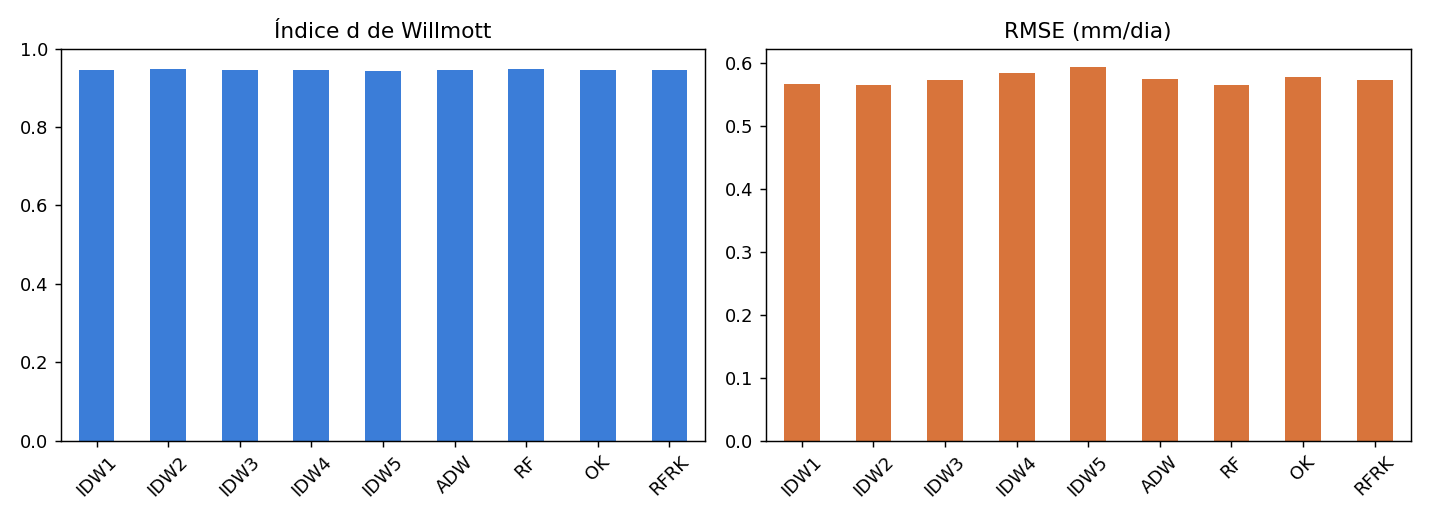
\includegraphics[width=\linewidth]{figuras/fig_metricas.png}
  \caption{Índice $d$ de Willmott (esq.) e RMSE (dir.) por método. As barras são
  visualmente quase iguais --- a evidência gráfica de que os interpoladores
  empatam.}
  \label{fig:metricas}
\end{figure}

\subsection{A significância das diferenças (Wilcoxon)}

A Tabela~\ref{tab:wilcoxon} compara o RFRK contra cada método pelo RMSE diário. O
RFRK é \emph{significativamente melhor} que a krigagem pura (OK) e que os IDW de
expoente alto (IDW4, IDW5), \emph{empata} com ADW e IDW3, e é
\emph{significativamente pior} que o RF --- porém por apenas \textbf{0,008~mm/dia}
de mediana. Esse é exatamente o ponto que o paper deixou em aberto: com milhares de
comparações diárias, diferenças minúsculas tornam-se ``significativas''. Em outras
palavras, \textbf{significância estatística não é o mesmo que relevância prática}.

\begin{table}[H]
  \centering
  \caption{Wilcoxon pareado: RFRK \emph{versus} cada método (RMSE diário). Diferença
  mediana $=$ med(RFRK) $-$ med(outro); negativo $\Rightarrow$ RFRK melhor.
  Significativo se $p<0{,}05$.}
  \label{tab:wilcoxon}
  \vspace{2pt}
  \begin{tabular}{lrrl}
    \toprule
    RFRK \emph{vs.} & Dif.\ mediana (mm/dia) & $p$-valor & Significativo \\
    \midrule
    RF   & $+0{,}008$ & $\approx 0$ ($10^{-20}$) & sim (RFRK pior) \\
    ADW  & $-0{,}009$ & 0,995    & não \\
    IDW1 & $-0{,}003$ & 0,038    & sim \\
    IDW2 & $-0{,}002$ & 0,037    & sim \\
    IDW3 & $-0{,}016$ & 0,386    & não \\
    IDW4 & $-0{,}024$ & 0,0004   & sim \\
    IDW5 & $-0{,}028$ & $\approx 0$ ($10^{-7}$) & sim \\
    OK   & $-0{,}026$ & 0,002    & sim \\
    \bottomrule
  \end{tabular}
\end{table}

\subsection{Mapas: os blocos do RF \emph{versus} a suavidade do RFRK}

A Figura~\ref{fig:mapas} mostra a ET\textsubscript{0} interpolada num dia de verão
e num de inverno, por IDW2, RF e RFRK. O RF produz uma superfície \emph{em degraus}
(``blocos''), artefato natural das árvores de decisão; o RFRK, ao reintroduzir a
estrutura espacial via krigagem dos resíduos, entrega um mapa visivelmente mais
suave. Embora não vença nas métricas, o RFRK tem \emph{menor viés} (BIAS $-0{,}019$
contra $-0{,}027$ do RF). O ganho do RFRK é, portanto, qualitativo (corrige o
artefato em blocos) mais do que numérico.

\begin{figure}[H]
  \centering
  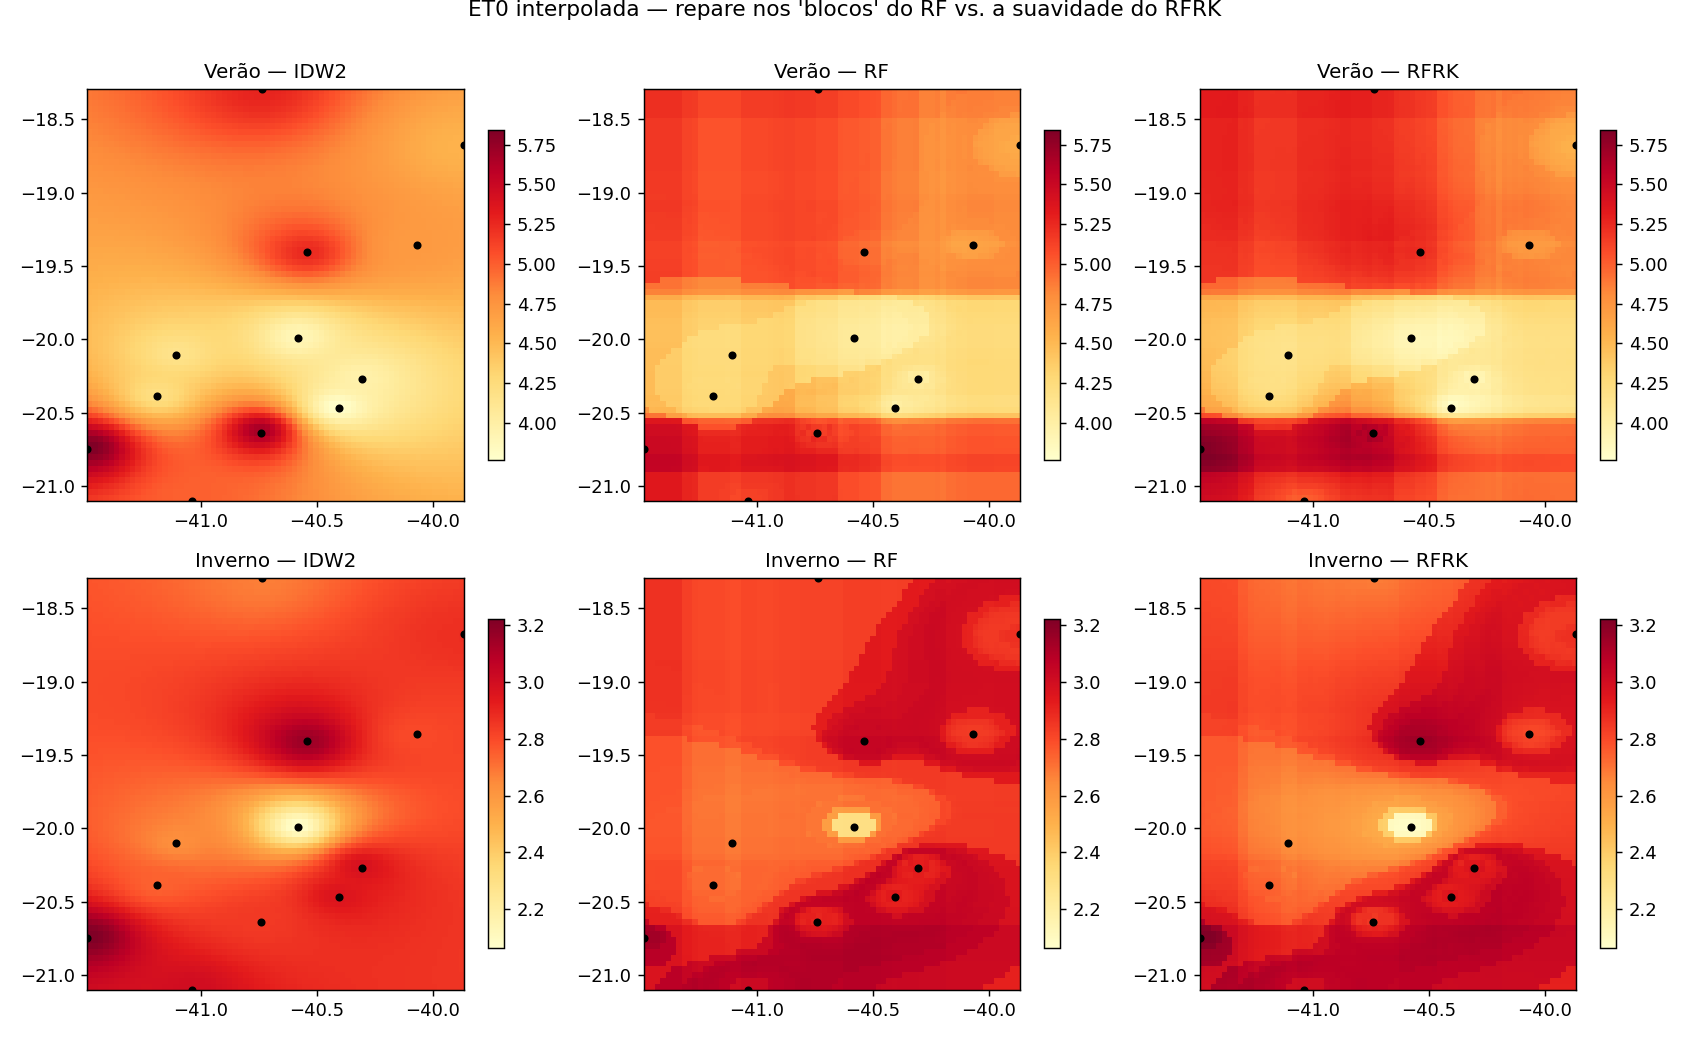
\includegraphics[width=\linewidth]{figuras/fig_mapas.png}
  \caption{ET\textsubscript{0} interpolada (mm/dia) em verão (linha superior) e
  inverno (inferior) por IDW2, RF e RFRK. Note os ``blocos'' do RF, em degraus,
  contra a suavidade do RFRK; pontos pretos são as estações.}
  \label{fig:mapas}
\end{figure}

\subsection{A habilidade do RF é sazonal, não espacial}

O resultado mais nítido é a importância de variáveis (Figura~\ref{fig:importancia}):
o \textbf{dia do ano responde por $\approx$87\%} da capacidade preditiva do RF, ao
passo que tudo o que é espacial (lon $+$ lat $+$ altitude) soma apenas $\approx$13\%
(doy $0{,}867$; alt $0{,}078$; lon $0{,}031$; lat $0{,}024$). Isso recontextualiza o
``detalhe espacial'' celebrado no paper: a força do RF vem majoritariamente de
capturar o \emph{ciclo sazonal} da ET\textsubscript{0}, não a estrutura espacial. E
explica por que o RFRK \emph{não} melhora as métricas --- como o resíduo do RF tem
pouca estrutura espacial a explorar, a krigagem dos resíduos tem pouco do que tirar
proveito.

\begin{figure}[H]
  \centering
  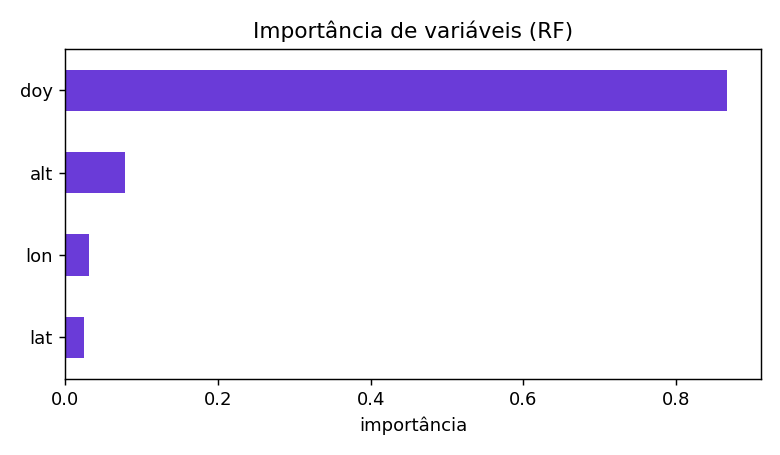
\includegraphics[width=0.72\linewidth]{figuras/fig_importancia.png}
  \caption{Importância de variáveis do RF (com o dia do ano, \texttt{doy}). O
  \texttt{doy} domina; lon, lat e altitude têm peso marginal.}
  \label{fig:importancia}
\end{figure}

A Figura~\ref{fig:scatter} reforça o ponto pelo lado sazonal: a dispersão
observado~$\times$~estimado é melhor no inverno ($d \approx 0{,}89$) do que no verão
($d \approx 0{,}84$), e o RF e o RFRK são praticamente sobreponíveis em ambas as
estações --- coerente com o achado de que sobra pouca estrutura espacial nos
resíduos.

\begin{figure}[H]
  \centering
  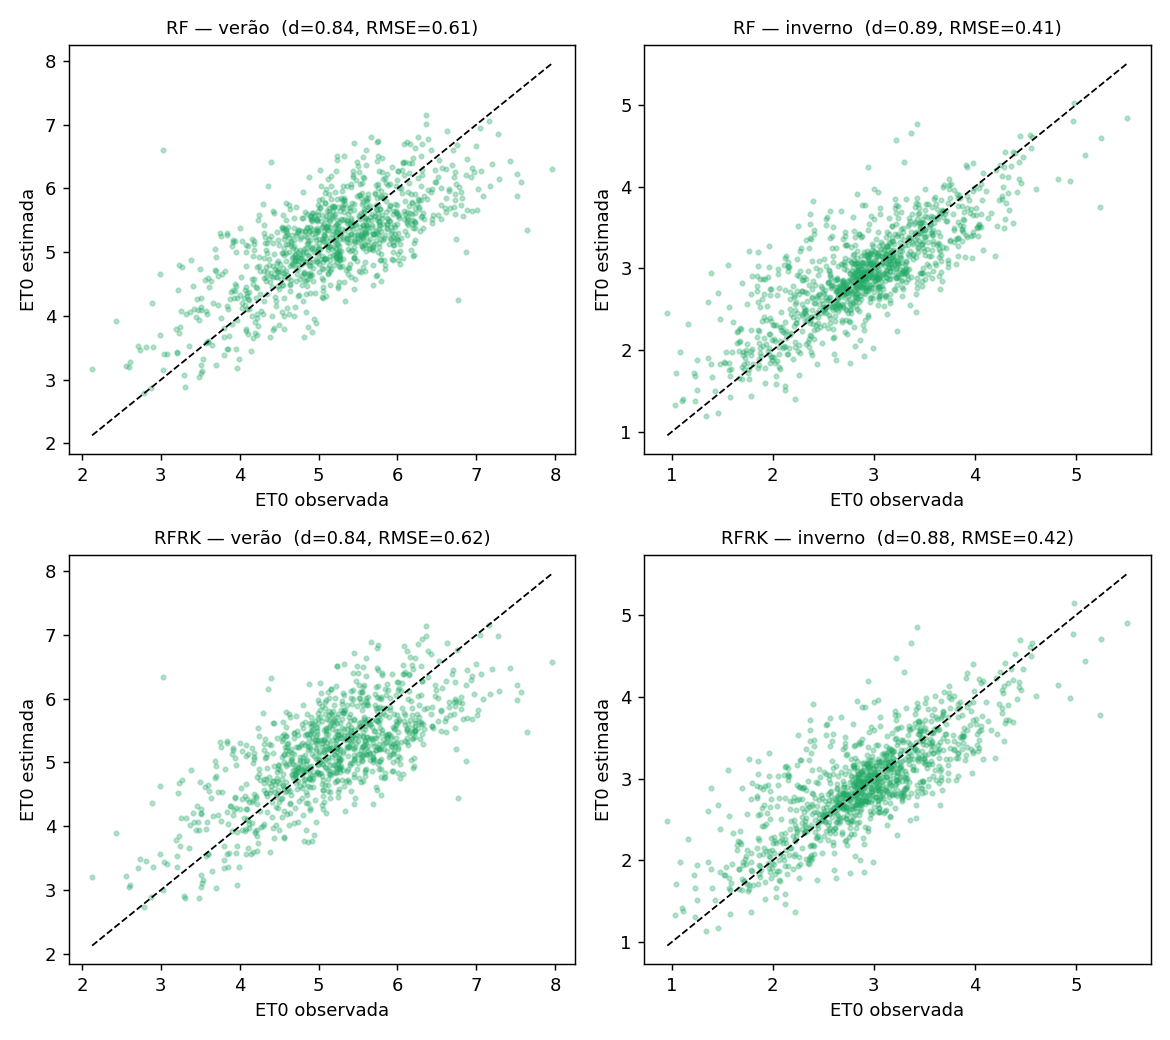
\includegraphics[width=0.62\linewidth]{figuras/fig_scatter.png}
  \caption{Observado $\times$ estimado para RF e RFRK, em verão e inverno. A linha
  tracejada é a identidade $1{:}1$; os rótulos trazem $d$ e RMSE por estação do ano.}
  \label{fig:scatter}
\end{figure}

% =====================================================================
\section{Desvios metodológicos assumidos}
% =====================================================================

O README do projeto explicita que o trabalho reproduz a metodologia, não os
números exatos do paper. Os desvios são: uso de estações automáticas do INMET em
vez das convencionais; ET\textsubscript{0} por Hargreaves--Samani em vez de
Penman--Monteith; covariáveis restritas a lon, lat e altitude; ADW na forma
canônica de New et al.; e OK com variograma exponencial fixo. Essas decisões
reduzem dependências externas e tornam o pipeline executável com dados abertos,
mas deslocam a comparação para o nível metodológico, e não para a reprodução
direta dos valores numéricos originais.

% =====================================================================
\section{Conclusão}
% =====================================================================

O projeto confirma, em uma reprodução metodológica aberta, que interpoladores
simples e modelos de aprendizado de máquina podem ficar numericamente muito
próximos na espacialização diária da ET\textsubscript{0}. O RF lidera por margem
pequena; IDW1/IDW2 permanecem competitivos; OK funciona como \emph{benchmark}
geoestatístico; e RFRK melhora a leitura visual dos mapas sem dominar as métricas
globais. Esse resultado reforça uma leitura importante do artigo-base: quando as
diferenças numéricas entre métodos são pequenas, a escolha do interpolador não
deve depender apenas de uma métrica agregada, mas também da estabilidade espacial
do mapa, do viés, da interpretabilidade e do custo de execução.

A contribuição mais forte está na integração: ingestão defensiva dos dados,
cálculo de ET\textsubscript{0}, LOO espacial, comparação de nove interpoladores,
Wilcoxon, importância de variáveis, MLflow, dashboard e Docker. Assim, a entrega
não fica restrita à reprodução isolada de uma tabela de resultados: ela organiza
um fluxo reprodutível, rastreável e executável de ponta a ponta, aproximando a
análise científica de uma solução de Machine Learning operacional. Trabalhos
futuros naturais são implementar Penman--Monteith, incluir DEM e variáveis
topográficas, ajustar variogramas por \emph{fold} e registrar formalmente um
modelo final versionado no MLflow.

% =====================================================================
\section*{Referências}
\addcontentsline{toc}{section}{Referências}
% =====================================================================
\sloppy

\refitem{Allen, R. G., Pereira, L. S., Raes, D., and Smith, M. (1998).
\textit{Crop evapotranspiration: guidelines for computing crop water
requirements}. FAO Irrigation and Drainage Paper 56, FAO, Rome.}

\refitem{Baratto, J., Wollmann, C. A., Iensse, A. C., and Roberti, D. R. (2022).
``Random forest for spatialization of daily evapotranspiration (ET0) in watersheds
in the Atlantic Forest''. \textit{Environmental Monitoring and Assessment},
194:449.}

\refitem{Breiman, L. (2001). ``Random forests''. \textit{Machine Learning},
45(1):5--32.}

\refitem{Hargreaves, G. H. and Samani, Z. A. (1985). ``Reference crop
evapotranspiration from temperature''. \textit{Applied Engineering in Agriculture},
1(2):96--99.}

\refitem{Hengl, T., Heuvelink, G. B. M., and Rossiter, D. G. (2007). ``About
regression-kriging: from equations to case studies''. \textit{Computers \&
Geosciences}, 33(10):1301--1315.}

\refitem{INMET --- Instituto Nacional de Meteorologia (2023). \textit{Dados
históricos das estações automáticas}.
\url{https://portal.inmet.gov.br/dadoshistoricos}.}

\refitem{New, M., Hulme, M., and Jones, P. (2000). ``Representing twentieth-century
space--time climate variability. Part II: development of 1901--96 monthly grids of
terrestrial surface climate''. \textit{Journal of Climate}, 13(13):2217--2238.}

\refitem{Pedregosa, F. et al.\ (2011). ``Scikit-learn: machine learning in
Python''. \textit{Journal of Machine Learning Research}, 12:2825--2830.}

\refitem{Wilcoxon, F. (1945). ``Individual comparisons by ranking methods''.
\textit{Biometrics Bulletin}, 1(6):80--83.}

\refitem{Willmott, C. J. (1981). ``On the validation of models''. \textit{Physical
Geography}, 2(2):184--194.}

\end{document}
